% 第 9 章 Using UPF and Power Analysis Tools
\bichapter{使用 UPF 与功耗分析工具}{Using UPF and Power Analysis Tools}
\label{chap:gui-upf}

对多电压设计，IC Compiler II GUI 提供 UPF 查看器、功耗状态表视图以及其他工具，用于查看设计的 UPF 功耗意图并支持分析。

本章包括以下主题：
\begin{itemize}
  \item 查看 UPF 功耗意图
  \item 查看功耗状态表
\end{itemize}

\section{查看 UPF 功耗意图}
\subsection*{Viewing the UPF Power Intent}

UPF 图以图形表示设计的 UPF 功耗意图，显示电源域（power domain）、供电网络、电源开关、隔离与保持策略，以及功耗意图中的其他元素。UPF 图支持缩放、平移、对象选择和对象查询。

选择 \textbf{View > Multivoltage UPF > Power Domain / Root Cell}，或单击 Power Domain 按钮。图~\ref{fig:gui-130} 同时显示版图、UPF 图和视图设置。

\begin{figure}[htbp]
\centering
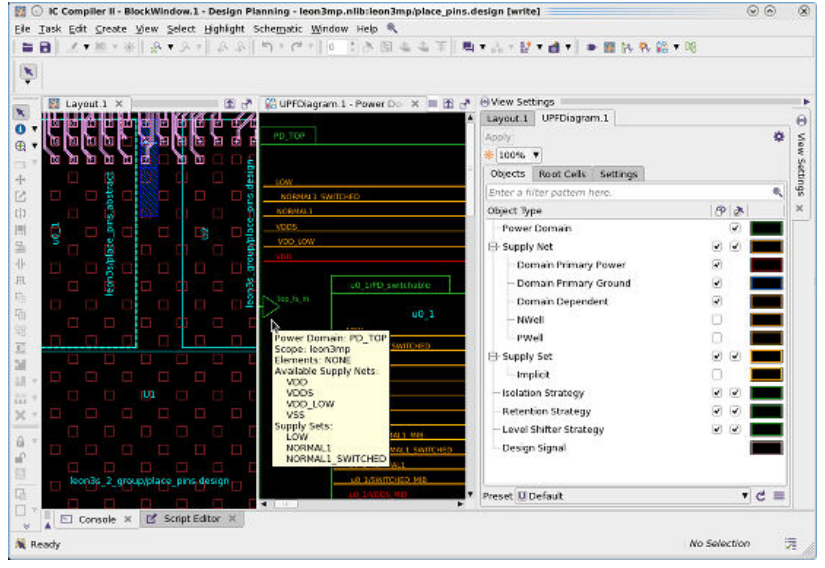
\includegraphics[width=0.92\textwidth]{gui-fig-130.png}
\caption{UPF 图视图}
\label{fig:gui-130}
\end{figure}

\subsection{电源域视图}
\subsubsection*{Power Domain View}

首次打开 UPF 图时，工具在电源域视图中显示 power scope 层次。信息按电源域层次组织。顶层电源域内的电源域显示为顶层的子模块。单击某个电源域即可选中它；右键可以选择相关单元、宏单元或 voltage area，也可以显示供电网络视图或功耗状态表。

每个电源域的供电集（supply set）画在矩形靠近顶部的位置；每条粗橙线代表一个唯一的供电集。单击该线即可选中。右键打开上下文菜单，选择 Show Supply Network View 或 Power State Table，可查看该供电集的更多信息。供电集下方是供电网络（supply net），每条细橙线代表一条供电网络。

用缩放和平移工具浏览视图，用方向键上下左右滚动。用选择工具点选单个对象，或框选矩形区域内的对象。指针停在对象上可在信息提示中预览；用 Query 工具可把对象信息显示在 Query 面板中。

在 View Settings 菜单中单击 UPFDiagram 选项卡，可查看电源域视图里对象类型与颜色的对应关系。单击色块可定制该对象类型的颜色。

若存在隔离单元，它们显示在供电网络下方。指针停在隔离单元上可在信息提示中看到更多信息。单击该线选中它，或右键打开上下文菜单，用以选择相关对象，或显示供电网络视图与功耗状态表。地网画在底部，每条细蓝线代表一条地网。

端口沿电源域边界显示。输入端口标为 I，输出端口标为 O。

\subsection{供电网络视图}
\subsubsection*{Supply Network View}

供电网络视图是电源域的另一种看法，显示不同电源域、隔离单元、开关单元以及电源域中其他元素之间的连接。与电源域视图一样，它按 power scope 层次组织。在视图中任意位置右键并选择 Show Supply Network View，即可显示图~\ref{fig:gui-131}。

\begin{figure}[htbp]
\centering
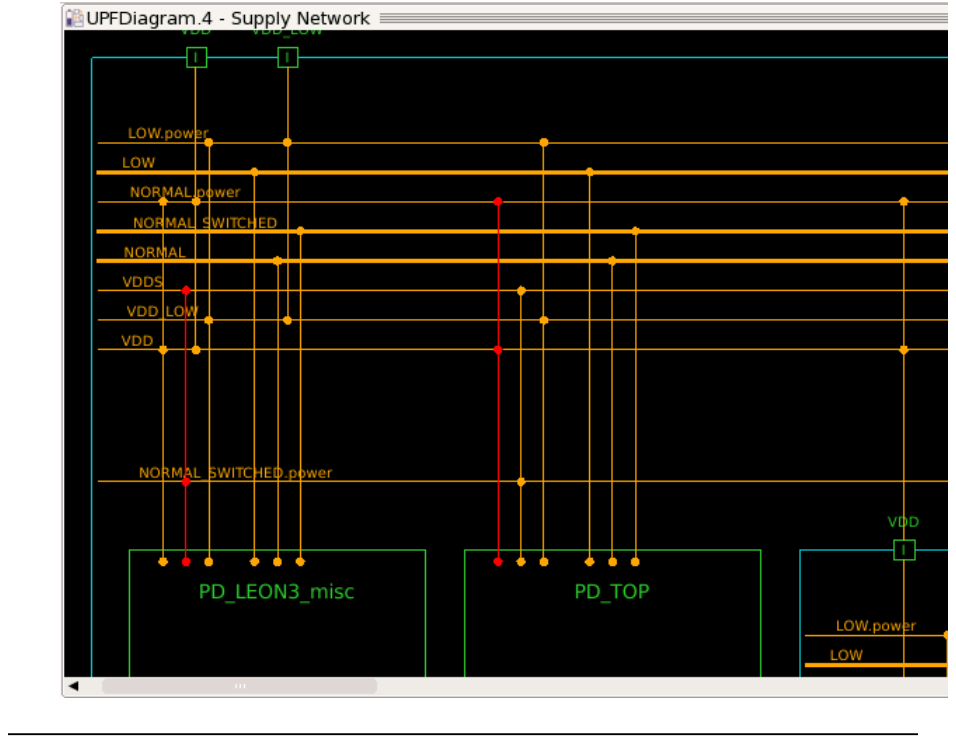
\includegraphics[width=0.92\textwidth]{gui-fig-131.png}
\caption{供电网络视图}
\label{fig:gui-131}
\end{figure}

\section{查看功耗状态表}
\subsection*{Viewing the Power State Table}

Power State Table 面板可与 UPF 图一起用来分析和调试隔离策略与电平移位策略。工具在功耗状态表中显示每路供电的状态，并在 UPF 图中显示它们的关系。面板见图~\ref{fig:gui-132}。

\begin{figure}[htbp]
\centering
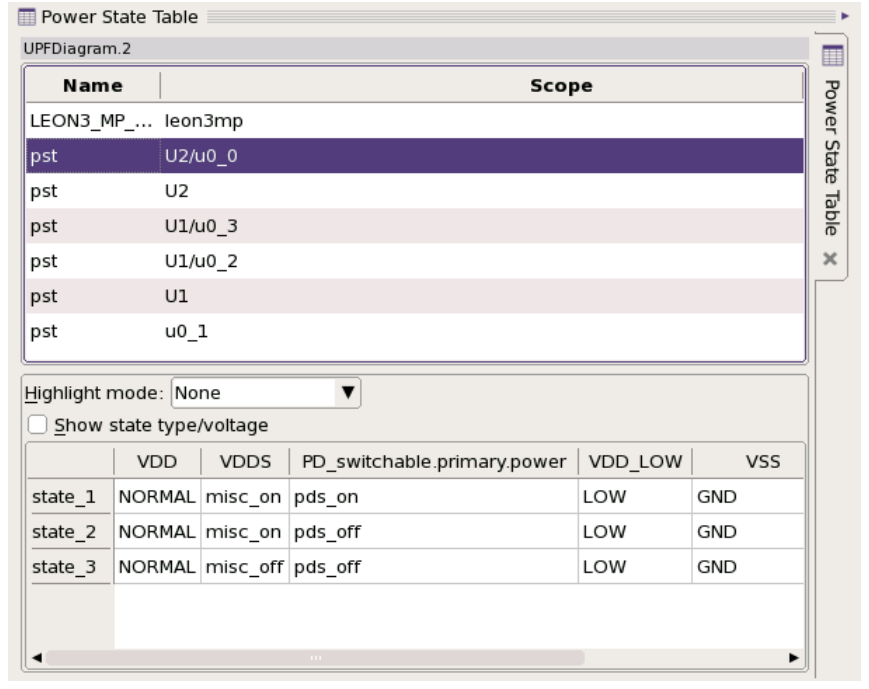
\includegraphics[width=0.92\textwidth]{gui-fig-132.png}
\caption{功耗状态表}
\label{fig:gui-132}
\end{figure}

该面板支持下列分析类型：
\begin{itemize}
  \item Always-on 分析比较电源与地之间的通断状态，结果为 More AO、Less AO、Equally AO 或 Unrelated AO 之一。
  \item 多电压电平移位分析比较各路电源之间的电压关系，结果为 LH（低到高）、HL（高到低）、HL\_LH（高低双向）或 None 之一。
\end{itemize}
